\documentclass{article}

\usepackage{algorithm2e}
\usepackage{amsmath}
\usepackage{amssymb}
\usepackage{amsthm}
\usepackage{authblk}
\usepackage[english]{babel}
\usepackage{blkarray}
\usepackage[font=small]{caption}
\usepackage{cite}
\usepackage{graphicx}

\setlength{\thickmuskip}{2mu plus 3mu minus 1mu}
\setlength{\medmuskip}{1mu plus 2mu minus 1mu}

\SetKwComment{Comment}{$\triangleright$\ }{}

% ---- Author affiliations ---- %

\renewcommand\Affilfont{\itshape\small}

% ---- Propositions, lemmas, defintions... ---- %

%\newtheorem{algorithm}{Algorithm}
\newtheorem{corollary}{Corollary}
\newtheorem{definition}{Definition}
%\newtheorem{example}{Example}
\newtheorem{lemma}{Lemma}
\newtheorem{proposition}{Proposition}
%\newtheorem{remark}{Remark}


% ---- Special environments (examples and remarks) ---- %

\newcounter{examplecounter}
\newenvironment{example}
{\small\vspace{0.5\baselineskip}
  \refstepcounter{examplecounter}%
  \noindent\textbf{Example \arabic{examplecounter}.}%
}{\vspace{-0.2\baselineskip}\begin{center}%
  $\star$\end{center}\vspace{0.5\baselineskip}}

\newcounter{remarkcounter}
\newenvironment{remark}
{\small\it\vspace{0.5\baselineskip}
  \refstepcounter{remarkcounter}%
  \noindent\textbf{Remark \arabic{remarkcounter}.}%
}{\vspace{0.5\baselineskip}}

\newenvironment{inset}
{\vspace{0.5\baselineskip}\begin{center}}
{\end{center}\vspace{0.5\baselineskip}}


% ---- Macros ---- %

\newcommand{\dn}[1]{\scriptstyle{\downarrow_{/#1}}}
\newcommand{\up}[1]{\scriptstyle{\uparrow_{/#1}}}
\newcommand{\nd}{\scriptstyle{|}}

%---------------------------------------------------------------

\title{Calibrating MEM seeding heuristics}

\author[1,2]{Guillaume J. Filion}
\author[1,2]{Eduard Zorita}
\affil[1]{Genome Architecture, Gene Regulation, Stem Cells and Cancer
Programme, Center for Genomic Regulation (CRG), The Barcelona Institute of
Science and Technology, Dr. Aiguader 88, Barcelona 08003, Spain.}
\affil[2]{University Pompeu Fabra, Doctor Aiguader, 08003 Barcelona,
Spain.}

\date{\today}

%---------------------------------------------------------------
%---------------------------------------------------------------


\begin{document}

\maketitle

\begin{abstract}
The abstract will come later.
A popular mapping heuristic is called \emph{seeding}, and a recent variant
is the \emph{MEM seeding} approach. Here we tackle the question of how to
evaluate the probability that MEM seeding hits are on-target. This in turn
expresses the confidence one should have in the location of the mapped DNA
fragment and can be used to calibrate the MEM seeding heuristic, or to
filter the hits at the desired level of confidence.
\end{abstract}


%---------------------------------------------------------------
%---------------------------------------------------------------

\section{Introduction}

\subsection{Mapping}

Consider the following task referred to as the \emph{true mapping
problem}: a random DNA fragment from a known genome is sequenced with an
imperfect instrument; can we identify the location of the fragment in the
genome?

It seems that the answer depends only on the size of the fragment and the
error rate of the instrument, but there is another important factor to
consider. Most genomes contain repeated sequences. Intuitively, the
problem is more difficult if the random DNA fragment is duplicated. If one
of the duplicates is exactly identical to the original, then the DNA
fragment cannot be mapped with certainty. Even if the duplicates are all
different from the original (which happens because of mutations in the
genome), the read may still be closer to one of the duplicates because of
sequencing errors. So we can never be sure that the read is mapped to the
\emph{true} location.

For this reason, we introduce the \emph{best mapping problem}, where we
search not the true, but the \emph{best} location of the DNA fragment,
\textit{i.e.} the sequence of the genome that is the most similar to the
read.

There are exact solutions to the best mapping problem, but the algorithms
are too slow to process the large amount of data generated by modern
sequencers. Instead, one uses heuristic methods, \textit{i.e.} algorithms
that run fast, but are not guaranteed to return the correct answer. In the
context of the best mapping problem, there are thus three possible
outcomes: $i.$ the DNA fragment is mapped to the best location, which is
called a \emph{true positive} (or an \emph{on-target hit}), $ii.$ the DNA
fragment is mapped to another location, which is called a \emph{false
positive} (or an \emph{off-target hit}), $iii.$ the DNA fragment is not
mapped at all, which is called a \emph{false negative}. A \emph{true
negative} would designate the outcome where a DNA fragment foreign to the
genome is not mapped at all, but here we assume that all DNA fragments
belong to the genome of interest.

In a seeding heuristic, one uses exact or near exact matches between the
read and the genome to collect a set of candidate locations. The read is
only compared to the sequences at the candidate locations, but not to the
rest of the genome. The advantage of this method is that there are few
candidates and that they can be discovered fast. However, the best hit may
not be in the candidate set, in which case it cannot be discovered
(\textit{i.e.}, the outcome is either a false positive or a false
negative).

A \emph{seed} designates a subsequence of fixed length that is shared
between the read and the genome. In other words, a seed is a perfect match
between a part of the read an a genomic site. The candidates consist of
the genomic sites that contain one or more seeds (this depends on the
specific heuristic).

In the theory developed below, we will assume that the \emph{true}
location of the read is also the \emph{best}. This is not always the case,
but it is unfeasible to model the behavior of the best hit in the present
context. We will later discuss how this relates to the probability that
the best hit has a seed.



\subsection{Maximal Exact Matches (MEMs)}

Here we consider a seeding variant where seeds do not have a fixed
length. Let us start by introducing the definition of a Maximal Exact
Match.

\begin{definition}
A Maximal Exact Match (MEM) is a subsequence of a read that is present in
the genome and that cannot be extended left or right --- either because
the read ends or because the extended subsequence is not in the genome.
\end{definition}

This definition presents a computational challenge: to know if a given
subsequence is a MEM, we need to know if it exists somewhere in the
genome. This is a non trivial problem in itself, but fortunately there
exists practical methods to answer the question, even for very large
genomes. Here on, we will assume that we always know which subsequences of
the read are MEMs.

A practical consideration is that short matches between the read and the
genome are irrelevant. For instance, $99.7\%$ of all the possible 12-mers
are present in the reference human genome, so an exact match of size 12 or
lower says nothing about the location of the DNA fragment. In what
follows, we will simply disregard short matches. More specifically, we
will assume that subsequences of the read can only match the original DNA
sequence or its duplicates, but not the rest of the genome. This will
simplify the discussion without loss of generality, because short
uninformative matches are ignored in all practical applications.

Fig.~\ref{fig:MEM_example} shows a concrete example of the relationship
between read errors, on-target matches, off-target matches and MEMs. The
sequence of the original DNA fragment is the first genomic hit (this is
the \emph{true} location). The second, third and fourth genomic hits are
duplicates. The mismatches between the genome and the read are
highlighted in bold. The read has three errors indicated by stars, so
\texttt{T}, \texttt{T} and \texttt{C} should actually be \texttt{A},
\texttt{A} and \texttt{G} (because the first hit is the \emph{true}
sequence).

\begin{figure}[h]
\centering
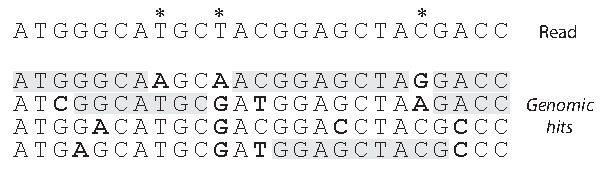
\includegraphics[scale=1]{MEM_example.pdf}
\caption{\textbf{Errors, matches and MEMs.}
Some legend.}
\label{fig:MEM_example}
\end{figure}

The MEMs are indicated by grey boxes. Technically, MEMs are subsequences
of the read, but they are shown on the genomic hits to highlight where
they match. Two MEMs can overlap, in which case they must match distinct
sequences of the genome (this follows from the definition). The last MEM
corresponds to two matches of length 4, with the first and the second
genomic hits. Such MEMs with several matches are referred to as
\emph{shared}. MEMs with a single match in the genome are referred to as
\emph{strict}.

As the name suggests, the principle of MEM seeding is to use MEM as seeds
to identify candidate genomic locations. Because short matches are
irrelevant, MEM seeds are usually requested to have a length greater than
or above a certain threshold denoted $\gamma$. We will assume that a
single MEM seed is sufficient to consider that a genomic hit is a
candidate location, which is why we will focus on the case that the read
does not have a single on-target MEM seed.

%In the example of Fig.~\ref{fig:MEM_example}, there is no MEM that matches
%the third genomic hit. It is important to understand that this can also
%happen to the best hit, as in the example shown in
%Fig~\ref{fig:MEM_eclipse}. The undesirable consequence is that some reads
%are bound to yield false positives, even if we tune the MEM seeding
%heuristic by changing the minimum seed length $\gamma$. We will refer to
%the case that the best hit is masked by off-target MEMs as \emph{MEM
%eclipse}. 
%
%\begin{figure}[h]
%\centering
%\includegraphics[scale=1]{MEM_eclipse.pdf}
%\caption{\textbf{MEM eclipse.}
%Some legend.}
%\label{fig:MEM_eclipse}
%\end{figure}
%
%If you are not already familiar with MEM seeding, we recommend that you
%take a moment to study the examples of Fig.~\ref{fig:MEM_example} and
%\ref{fig:MEM_eclipse}. This will be essential to understand the next
%sections. Before reading further, make sure that you can answer the
%following questions:
%\begin{enumerate}
%\itemsep0em
%\item What are the conditions for a MEM to be shared?
%\item What is the minimum number of duplicates for MEM eclipse?
%\end{enumerate}


\section{Combinatorial construction of reads}

In this section we give a representation of reads as combinatorial ojects.
The construction has two essential purposes: the first is to give a
generative model of reads without any on-target MEM seed, the second is to
allow us to find their weighted generating function, which in turn will
allow us to find their probability of occurrence.

\subsection{The MEM alphabet}

The nucleotide sequence of the read is not so useful to know where MEMs
are and whether they are on-target. To develop a formal method to compute
the probability that the read contains an on-target MEM seed, we will
recode reads as sequences of letters from the so-called \emph{MEM
alphabet} $\{\downarrow, \uparrow, \square\}$.

Each nucleotide of the read is recoded with one of three letters. The
$\downarrow$ symbol indicates that the nucleotide is a sequencing error.
By definition, it is a mismatch for the target. The $\uparrow$ symbol
characterizes the presence of an on-target MEM in a way that we are about
to clarify. All the other nucleotides are represented by the $\square$
symbol.

To understand the meaning of the $\uparrow$ symbol, consider the following
situation: at the left end of the read, as we try to extend the first
match as much as possible to the right, the number of hits in the genome
keeps decreasing. It may be the case that at some point, we are left with
a single hit that is on-target. The very first nucleotid where that
happens is called the \emph{pivot} and is labelled with the symbol
$\uparrow$.

Fig.~\ref{fig:sketch_MEM} shows the read of Fig.~\ref{fig:MEM_example} as
encoded with the MEM alphabet. Below the read are the matches between the
read and the genomic hit, as they are in Fig.~\ref{fig:MEM_example}. A
black square means that the nucleotide is a mismatch for the genomic
sequence, and a white or grey square means that it is a match. Grey
squares are used to highlight MEMs, as in Fig.~\ref{fig:MEM_example}.


\begin{figure}[h]
\centering
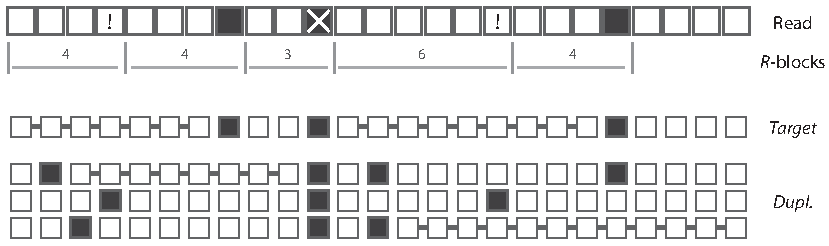
\includegraphics[scale=.85]{sketch_MEM.pdf}
\caption{\textbf{Reads and MEM seeds}. 
Some legend.}
\label{fig:sketch_MEM}
\end{figure}

Observe that the two on-target MEMs contain a pivot, but the shared MEM
does not. This is always the case. Recall that the pivot indicates that
the true location is the \emph{only} local match, so the $\uparrow$ symbol
cannot appear in on-target MEM seeds when they are shared.

Strict on-target MEM seeds are easy to find when reads are represented in
the MEM alphabet: they are the longest stretches of symbols containing the
$\uparrow$ symbol and not containing the $\downarrow$ symbol. Shared
on-target MEM seeds are trickier. They do not directly appear in this
representation so we will have to keep that in mind throughout the theory.
It is in a sense justified to put more emphasis on strict MEM seeds
because they guarantee that the true location will be found. Shared MEM
seeds can have thousands of hits in the genome in practice, so the user
may not test them all. That said, the theory developed here fully takes
shared MEM seeds into account, even if they are not visible in the
representation of the MEM alphabet.

The point of the MEM seeding alphabet is that reads can be seen as
sequences of letters, but also as sequences of \emph{segments} delimited
by the $\uparrow$ and the $\downarrow$ symbols. Because such segments are
intimately linked to the presence of on-target MEM seeds, we can give a
construction of reads that do not contain any.

\begin{definition}
\label{def:segment}
A segment is a sequence of $\square$ symbols terminated by either a
$\uparrow$ symbol or by a $\downarrow$ symbol. The unterminated sequence
of $\square$ symbols at the end of the read is called the tail --- which
can thus be an empty sequence of symbols.
\end{definition}

Following definition~\ref{def:segment}, the $\uparrow$ and $\downarrow$
symbols will be referrred to as \emph{terminators}.
Fig.~\ref{fig:sketch_segment} shows the decomposition of the read from
Fig.~\ref{fig:sketch_MEM} in segments. The size of each segment (the
number of nucleotides that compose it) is indicated below.

\begin{figure}[h]
\centering
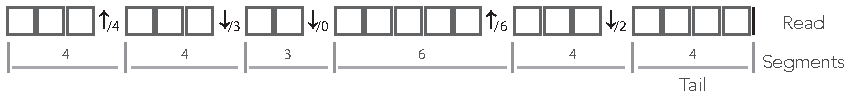
\includegraphics[scale=.85]{sketch_segments.pdf}
\caption{\textbf{Reads as sequences of segments}. 
Some legend.}
\label{fig:sketch_segment}
\end{figure}


\subsection{The extended MEM alphabet}

An issue with the MEM alphabet is that the probabilities of the symbols
are difficult to evaluate. The $\downarrow$ symbol coincides with read
errors, which is straightforward to model. The $\uparrow$ symbol coincides
with pivots, which have a more complex behavior. We thus extend the MEM
alphabet so that the occurrence of the $\uparrow$ becomes easier to
evaluate.

Only the terminators are extended; the $\square$ symbols remain unchanged.
Let us denote the number of duplicates of the target by $N$. The
$\downarrow$ symbol is replaced by the $N+1$ symbols
$\downarrow_{/m}$, where $m$ is the number of duplicates that
\emph{match} the erroneous nucleotide $(0 \leq m \leq N)$. The $\uparrow$
symbol is replaced by the symbols $\uparrow_{/j}$, where $i
\geq 0$ is the size of the segment (including the
$\uparrow_{/j}$ symbol). Finally, we add the special terminator
$|$ that marks the end of the read. In other words, tails are considered
normal segments terminated by the symbol $|$ (with size 0).

It is important to highlight that the numbers that decorate the symbols
have a very different nature. In the case of the $\downarrow$ symbol, it
is an information about the number of sequences matching the read; in the
case of the $\uparrow$ symbol, it is the position of the pivot relative to
the previous terminator (or to the beginning of the read).

Fig.~\ref{fig:sketch_extended} shows the decomposition of the read from
Fig.~\ref{fig:sketch_segment} in segments using the extended MEM alphabet.
The numbers decorating the symbols are shown above them to avoid crowding
the figure.

\begin{figure}[h]
\centering
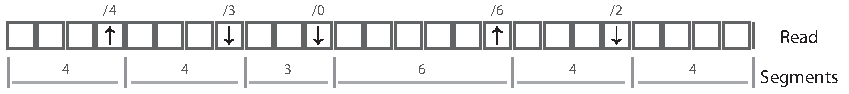
\includegraphics[scale=.85]{sketch_extended.pdf}
\caption{\textbf{Reads as sequences of segments in the extended MEM
alphabet}. 
Some legend.}
\label{fig:sketch_extended}
\end{figure}

There is an infinite amount of $\uparrow_{/j}$ symbols in the
extended MEM alphabet, but if the read has no on-target MEM seed, then
only the $\uparrow_{/j}$ symbols where $1 \leq i \leq \gamma-1$
can be used (if a pivot terminates a segment of size greater than or equal
to $\gamma$, then the read contains a strict on-target MEM seed). The
extended MEM alphabet is made in such a way that the numbers decorating
the $\uparrow$ symbol will allow us to exclude strict on-target MEM seeds,
and the numbers decorating the $\downarrow$ symbol will help us exclude
shared on-target MEM seeds.


\section{Symbolic and analytic representations}

\subsection{Weighted generating functions}

Let $\mathcal{A}$ be a set of combinatorial objects which have a
\emph{probability of occurrence}, and a \emph{size} that is an integer
number. The function defined as $A(z) = \sum_{k=0}^\infty a_kz^k$, where
$a_k$ is the total probability of objects of size $k$, is called the
\emph{weighted generating function} of the combinatorial objects.

In our case, we are interested in the weighted generating function of
reads without on-target MEM seed, where the coefficient $a_k$ is the
probability that a read of size $k$ has no on-target MEM seed. As $k$
becomes larger, it becomes more difficult to evaluate $a_k$, but the
combinatorial construction developed above will allow us to do this by
using established strategies involving weighted generating functions.


\subsection{The symbolic method}

The symbolic method is a strategy belonging to the general \emph{analytic
combinatorics} framework. The idea is to combine simple combinatorial
objects into more complex objects. Each combinatorial operation on the
objects corresponds to a mathematical operation on their weighted
generating functions. One can thus obtain the weighted generating function
of complex objects, and from there extract their probability of
occurrence.

The combinatorial construction of reads using the extended MEM seeding
alphabet gives us a method to express their weighted generating function
from that of segments. More specifically, we can describe complex
sequences of segments through a so-called \emph{transfer matrix} $M(z)$
that specifies which segments can follow one another in the reads of
interest.

The segments types are identified by their terminators and arranged in a
predefined oder. The entry of $M(z)$ at coordinates $(i,j)$ is the
weighted generating function of segments with the $j$-th terminator that
can be inserted immediately after segments with the $i$-th terminator. The
matrix $M(z) + M(z)^2 + \ldots = M(z) \cdot (I-M(z))^{-1}$ contains the
weighted generating functions of the reads of all sizes. The entry that
corresponds to terminators $\downarrow_{/0}$ and $|$ is the weighted
generating function of the reads of interest (the beginning of the read is
equivalent to a ghost segment terminated by $\downarrow_{/0}$,
\textit{i.e.} a mismatch for all the sequences).

With the transfer matrix $M(z)$, with thus have a way of computing the
weighted generating function of the reads without on-target MEM seed, and
from there we can extract teir probability of occurrence. Our next task is
thus to specify $M(z)$.



\section{The transfer matrix}

\subsection{Match streak and masks}

For each sequence, we define the \emph{match streak} at a given nucleotide
as the number of nucleotides since the last mismatch on the left. For
instance, in Fig.~\ref{fig:MEM_example}, the match streak of the first
genomic hit at the ninth nucleotide is $1$ while for the second genomic
hit, it is $7$.

\begin{definition}
At a given position of the read, a duplicate sequence is a \emph{hard
mask} if its success streak is strictly longer than the match streak of
the target. A duplicate thread is a \emph{soft mask} if its has the same
match streak as the target.
\end{definition}

For instance, the second genomic hit in the example above is a hard mask
at the ninth nucleotide. The point of hard and soft masks is that they are
directly linked with MEMs. A nucleotide with a hard mask cannot belong to
an on-target MEM. A nucleotide without mask belongs to a strict on-target
MEM. A nucleotide with a soft mask may belong to a strict on-target MEM,
to a shared on-target MEM, or may not belong to any MEM. The distinction
between the three cases will be clarified in the specification of the
transfer matrix.

The extended MEM alphabet is nothing more than a way to keep track of the
hard and soft masks. For instance, a pivot (associated with the symbol
$\uparrow$) is a nucleotide where the number of masks becomes is reduced
to 0. If there are $N$ duplicates, the symbol $\downarrow_{/m}$ indicates
that there $m$ hard masks and $N-m$ soft masks.


\subsection{Error model and divergence of the duplicates}

We assume that the target sequence has $N$ duplicates. We further assume
that duplication was instantaenous and that all $N+1$ sequences diverge
independently from each other at a constant rate. In other words, we
ignore the complications due to the genealogy of the duplication events
and we simply assume that at each position, any given duplicate is
identical to the target with probability $1-\mu$. If it is not, we
assume that the duplicate has any of the remaining three nucleotides with
equal probability (\textit{i.e.} each is found with probability $\mu/3$).

We also assume that the sequencing instrument has a constant substitution
rate $p$, and that insertions and deletions never occur. In case of a
substitution, we again assume that the remaining three nucleotides are
equally likely.

On a read error the target is never identical to the read (because we
assume that the target is the true sequence), and a duplicate is identical
to the read with probability $mu/3$ (the probability that the duplicate is
different from the target, times the probability that the nucleotide is
the same as the error). On a correct nucleotide, the target is always
identical to the read, and a dupicate is identical with probability
$1-\mu$ (the probablity that the duplicate is identical to the target).

With these assumptions, we are now ready to describe the entries of the
transfer matrix $M(z)$, which we do in order of increasing difficulty.


\subsection{Segments following $\uparrow_{/j}$}

A $\uparrow_{/j}$ symbol marks a pivot and the absence of masks. The
segment is thus the beginning of an on-target MEM of size at least $j$.
The MEM will extend until the next sequencing error, or until the end of
the read, so the number of $\square$ symbols in the next segment must be
at most $\gamma-j-1$ and it must be terminated by a $\downarrow$ symbol or
by the tail terminator $|$.

In this case, the matches between the read and the duplicates are
irrelevant until the terminator. The weighted genearting function of each
$\square$ symbol is simply $qz$ ($q$ is the probability that the
nucleotide is not an error and $z$ marks objects of size $1$).

\begin{definition}
The probability that a symbol is $\downarrow_{/m}$ given that the
nucleotide is a read error is
\begin{equation}
\label{eq:omega}
\omega_m = {N \choose m} \big(1 - \mu/3\big)^{N-m} \big(\mu/3\big)^m.
\end{equation}
\end{definition}

The weighted generating function of the $\downarrow_{/m}$ terminator is
thus $\omega_m pz$ (the probability of the $\downarrow_{/m}$ is $\omega_m
p$ and $z$ marks objects of size $1$).

The entries of the transfer matrix that correspond to transitions from
$\uparrow_{/j}$ to other segments are now easy to find. The weighted
generating function of the segments terminated by $\downarrow_{/m}$
following a segment terminated by $\uparrow_{/j}$ is
\begin{equation}
\label{eq:D}
D_{j,m}(z) = \omega_m pz \sum_{i=0}^{\gamma-j-1} (qz)^i.
\end{equation}

And the weighted generating function of the tail segments following
segments terminated by $\uparrow_{/j}$ is
\begin{equation}
\label{eq:E}
E_j(z) = \sum_{i=0}^{\gamma-j-1} (qz)^i.
\end{equation}


\subsection{Segments following $\downarrow_{/m}$}

At a $\downarrow_{/m}$ symbol, there are $m$ hard masks and $N-m$ soft
masks. If all the masks disappear before the first read error, the next
terminator will be a $\uparrow$ symbol, otherwise it will be a
$\downarrow$ symbol.

\subsubsection*{Case 1: the terminator is $\uparrow_{/i}$}

\begin{definition}
The probability that a given duplicate sequence contains a mismatch in a
sequence of $i$ error-free nucleotides is
\begin{equation}
\label{eq:xi}
\xi_i = 1-(1-\mu)^i.
\end{equation}
\end{definition}

With this notation, the probability that at least one mask survives a
sequence of $i$ error-free nucleotides is thus $1-\xi_i^N$, and the
probability that there remains a mask at the $i-1$-th but not at the 
$i$-th error-free nucleotide is $\xi_i^N - \xi_{i-1}^N$. From this we
conclude that the weighted generating function of the segments terminated
by $\uparrow_{/i}$ following a segment terminated by $\downarrow_{/m}$ is
\begin{equation}
\label{eq:B}
B_i(z) = \Big( \xi_i^N-\xi_{i-1}^N \Big) (qz)^i.
\end{equation}

In the equation above, $q^i$ is the probability that there is no
sequencing error in $i$ nucleotides and $z^i$ marks objects of size $i$.
As mentioned above, $i < \gamma$ for reads without on-target MEM seed.
Also note that this expression is the same for all $\downarrow$ symbols;
it does not depend on $m$.

\subsubsection*{Case 2a: the terminator $|$ comes before the $\gamma$-th
nucleotide}

In this case there can be no on-target MEM seed. We must just enforce the
condition that at least one of the $N$ masks survives until the end of the
segment in order to exclude the $\uparrow$ symbol. The weighted generating
function is
\begin{equation*}
\sum_{i=0}^{\gamma-1} \Big(1 - \xi_i^N \Big) (qz)^i.
\end{equation*}

\subsubsection*{Case 2b: the terminator $|$ comes after the $\gamma$-th
nucleotide}

In this case, the soft masks are irrelevant. Even if they survive until
the end of the segment, there will be a shared on-target MEM seed. So we
must enforce the condition that at least one hard mask survives until the
end of the segment (which is impossible if $m = 0$).
\begin{equation*}
\sum_{i=\gamma}^\infty \Big(1 - \xi_i^m \Big) (qz)^i.
\end{equation*}

The transition from $\downarrow_{/m}$ to $|$ is
\begin{equation}
\label{eq:C}
C_m(z) =
\sum_{i=0}^{\gamma-1} \Big(1 - \xi_i^N \Big) (qz)^i +
  \sum_{i=\gamma}^\infty \Big(1 - \xi_i^m \Big) (qz)^i.
\end{equation}

\subsubsection*{Case 3a: the terminator $\downarrow_{/n}$ comes before the
$\gamma$-th nucleotide}

As above, there can be no on-target MEM seed and we must just exclude the
$\uparrow$ terminator. The weighted generating function is
\begin{equation}
\omega_n pz \sum_{i=0}^{\gamma-1} \Big(1 - \xi_i^N \Big) (qz)^i.
\end{equation}

\subsubsection*{Case 3a: the terminator $\downarrow_{/n}$ comes after the
$\gamma$-th nucleotide}

This case is by far the most convoluted. Since the segment contains at
least $\gamma$ error-free nucleotides, we must take care that it does not
generate an on-target MEM seed. This will be the case if any of the two
following conditions is validated: $i)$ at least one hard mask covers all
the error-free nucleotides, or $ii)$ none of the hard masks does but at
least one soft mask covers the whole segment (including the terminator).

The two conditions are mutually exclusive by construction. They are
graphically represented in the diagram below. The left panel corresponds
to case $i)$ and the panel to case $ii)$. The top row represents the
target, and the bottom rows represent duplicates (using the same
symbols as in Fig.~\ref{fig:sketch_MEM}).
\begin{inset}
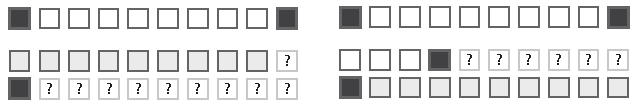
\includegraphics{masks.pdf}
\end{inset}

Whenever a hard mask (here the first duplicate) covers the nucleotides
as shown in the left panel, there can be no on-target MEM seed,
irrespective of the value of $\gamma$. The positions marked with a
question mark are irrelevant, they cannot change the fact that there is no
on-target MEM seed. If the hard masks are interrupted, as in the right
panel, then it depends on the soft masks. If a soft mask covers the whole
segment, then there can be no on-target MEM seed, irrespective of the
value of $\gamma$.

Condition $i)$ has probability $\big(1 - \xi_i^m \big)$ and the
weighted generating function is thus
\begin{equation*}
\omega_n pz \sum_{i=\gamma}^\infty \Big(1 - \xi_i^m \Big) (qz)^i.
\end{equation*}

For condition $ii)$, we will need to introduce some new notations.
\begin{definition}
The probability that a given duplicate sequence contains a mismatch in a
sequence of $i$ error-free nucleotides followed by an error is
\begin{equation}
\label{eq:eta}
\eta_i = 1-(1-\mu)^i\mu/3.
\end{equation}
\end{definition}

The probability of condition $ii)$ is
\begin{equation*}
\xi_i^m \Big(1 - \eta_i^{N-m} \Big),
\end{equation*}
but we need to break up this term among the terminators $\downarrow_{/n}$,
($0 \leq n \leq N$). For this, we decompose the sum on the number of soft
masks that run to the end of the segment, including the terminator. The
probability that there are $r \geq 1$ such soft masks is
\begin{equation*}
{N-m \choose r} (1 - \eta_i)^r \eta_i^{N-m-r}.
\end{equation*}

Each of them matches the nucleotide at the end of the segment, so the
total number of matches is $r$ plus the number of sequences, among the
remaining $N-m-r$ soft masks and $m$ hard masks, that also match the
last nucleotide.

Let us start with the $N-m-r$ that failed somewhere in the segment. The
conditional probability that they match the last nucleotide given that
they fail somewhere in the segment is $\mu/3 \cdot \xi_i / \eta_i$. The
conditional probability that they do not match is $(1-\mu/3) / \eta_i$.
For the $m$ hard masks, the probability that they match the last
nucleotide given that they sail somewhere in the segment is simply
$\mu/3$, and the probability that they do not is $1-\mu/3$.

The probability that those $N-r$ duplicates contribute $n-r$ matches is
\begin{equation*}
\frac{(\mu/3)^{n-r}(1-\mu/3)^{N-n}}{\eta_i^{N-m-r}}
\psi_{i,m,n,r}\text{, where \;}
\psi_{i,m,n,r} = \sum_{q \geq 0}{m \choose q}{N-m-r \choose n-r-q}
\xi_i^{n-r-q}.
\end{equation*}


The probability that in
total $n$ sequences match the terminator is
\begin{eqnarray*}
&\;& \sum_{r\geq1} {N-m \choose r}
(1 - \eta_i)^r (\mu/3)^{n-r} (1-\mu/3)^{N-n} \psi_{i,m,n,r} \\
&=& (\mu/3)^n(1-\mu/3)^{N-n} \sum_{r\geq1} {N-m \choose r}
  (1 - \mu)^{ri} \psi_{i,m,n,r} \\
&=& \omega_n \cdot \zeta_{i,m,n},
\end{eqnarray*}
where
\begin{equation}
\label{eq:zeta}
\zeta_{i,m,n} = \sum_{r\geq1} {N-m \choose r}
(1-\mu)^{ri} \psi_{i,m,n,r} \bigg/ {N \choose n}.
\end{equation}


The weighted generating function we are looking for is thus
\begin{equation}
\label{eq:A}
A_{m,n} =
\omega_n pz \sum_{i=0}^{\gamma-1} \Big(1 - \xi_i^N \Big) (qz)^i + \omega_n
pz \sum_{i=\gamma}^\infty \Big(1 - \xi_i^m \cdot
(1- \zeta_{i,m,n}) \Big) (qz)^i.
\end{equation}

\subsection{The expression of the transfer matrix}

The final expression for the transfer matrix $M(z)$ is
\begin{equation*}
\begin{blockarray}{cccccccc}
   & \dn{0} & \ldots & \dn{N} & \up{1} & \ldots & \up{\gamma-1} & \nd \\
\begin{block}{c[ccccccc]}
\dn{0} & A_{0,0}(z) & \ldots & A_{0,N}(z) & B_1(z) & \ldots &
    B_{\gamma-1}(z) & C_0(z) \\
\vdots & \vdots & \ddots & \vdots & \vdots & \ddots &
    \vdots & \vdots \\
\dn{N} & A_{N,0}(z) & \ldots & A_{N,N}(z) & B_1(z) & \ldots &
    B_{\gamma-1}(z) & C_N(z) \\
\up{1} & D_{1,0}(z) & \ldots & D_{1,N}(z) & 0 & \ldots & 0 & E_1(z) \\
\vdots & \vdots & \ddots & \vdots & \vdots & \ddots &
    \vdots & \vdots \\
\up{\gamma-1} & D_{\gamma-1,0}(z) & \ldots & D_{\gamma-1,N}(z) & 0 &
  \ldots & 0 & E_{\gamma-1}(z) \\
\nd & 0 & \ldots & 0 & 0 & \ldots & 0 & 0 \\
\end{block}
\end{blockarray}
\end{equation*}
where
\begin{gather}
\tag{\ref{eq:A}}
A_{m,n} =
\omega_n pz \sum_{i=0}^{\gamma-1} \Big(1 - \xi_i^N \Big) (qz)^i + \omega_n
pz \sum_{i=\gamma}^\infty \Big(1 - \xi_i^m \cdot
(1- \zeta_{i,m,n}) \Big) (qz)^i \\
\tag{\ref{eq:B}}
B_i(z) = \Big( \xi_i^N-\xi_{i-1}^N \Big) (qz)^i \\
\tag{\ref{eq:C}}
C_m(z) =
\sum_{i=0}^{\gamma-1} \Big(1 - \xi_i^N \Big) (qz)^i +
  \sum_{i=\gamma}^\infty \Big(1 - \xi_i^m \Big) (qz)^i \\
\tag{\ref{eq:D}}
D_{j,m}(z) = \omega_m pz \sum_{i=0}^{\gamma-j-1} (qz)^i \\
\tag{\ref{eq:E}}
E_j(z) = \sum_{i=0}^{\gamma-j-1} (qz)^i
\end{gather}
and where
\begin{gather}
\tag{\ref{eq:omega}}
\omega_m = {N \choose m} \big(1 - \mu/3\big)^{N-m} \big(\mu/3\big)^m \\
\tag{\ref{eq:xi}}
\xi_i = 1-(1-\mu)^i \\
\tag{\ref{eq:eta}}
\eta_i = 1-(1-\mu)^i\mu/3 \\
\tag{\ref{eq:zeta}}
\zeta_{i,m,n} = \sum_{r\geq1} {N-m \choose r}
(1-\mu)^{ri} \psi_{i,m,n,r} \bigg/ {N \choose n} \\
\notag
\psi_{i,m,n,r} = \sum_{q \geq 0}{m \choose q}{N-m-r \choose n-r-q}
\xi_i^{n-r-q}.
\end{gather}


\section{Computing the probabilities}

\subsection{Coefficient extraction}

The purpose of constructing the weighted generating function $F(z) = a_0 +
a_1z + a_2z^2 + \ldots$ is to extract the coefficient $a_k$, which
represents the probability that a read of size $k$ does not contain an
on-target MEM seed. $F(z)$ is the entry at coordinates $(1,N+\gamma+1)$ of
the matrix $M(z) \cdot (I-M(z))^{-1}$. The expression of $M(z)$ is in
general too complex to compute this function directly. Instead, we return
to the expression $M(z) \cdot (I-M(z))^{-1} = M(z) + M(z)^2 + \ldots$ and
observe that the terms $M(z)^{k+2}, M(z)^{k+3}, \ldots$ have no influence
on the coefficients $a_0, a_1, \ldots, a_k$.

Indeed, a read of size $k$ has at most $k+1$ segments. Since the entries
of $M(z)^k$ are the weighted generating functions of reads with exactly
$k$ segments, $a_k$ cannot depend on $M(z)^{k+2}, M(z)^{k+3}$. More
formally, we can prove by induction that all the entries of $M(z)^k$ are
divisible by $z^{k-1}$, showing that the contribution of $M(z)^{k+2} +
M(z)^{k+3} + \ldots$ to $a_0 + a_1z + \ldots +a_kz^k$ is $0$.

So we can extract the coefficients of $F(z)$ up to order $k$ by computing
the matrix $M(z) + M(z)^2 + \ldots + M(z)^{k+1}$, and compute the first
terms of the Taylor expansion of the entry at coordinates
$(1,N+\gamma+1)$.

But we can do better than that. If we are only interested in the
coefficients of order up to $k$, we can replace the infinite power series
of the terms $A_{m,n}(z)$ and $C_m(z)$ by their truncated versions where
we keep only the terms of order up to $k$. Likewise, we perform all
algebraic operation on truncated polynomials of order $k$, \textit{i.e.}
we discard at every stage the coefficients of order greater than $k$. With
this approach, the entry of the matrix $M(z) + M(z)^2 + \ldots +
M(z)^{k+1}$ at coordinates $(1,N+\gamma+1)$ is a truncated polynomial that
directly provides the coefficients of interest.

But we can do better than that. A read with $k$ segments contains at least
$(k-1)/2$ errors. Indeed, two segments terminated by $\uparrow$ cannot
follow each other, so at least (approximately) half of the segments must
be terminated by $\downarrow$, which means that the segment contains a
read error. Since read errors typically have a small probability of
occurrence, all the coefficients of $M(z)^k$ rapidly converge to $0$ and
become negligible as $k$ increases. So instead of computing $M(z) + M(z)^2
+ \ldots + M(z)^{k+1}$, we can interrupt the summation after a certain
power of $M(z)$ because the terms are negligible.

This approach makes it feasible to compute the probability that a read of
size $k$ has no on-target MEM seed when the matrix $M(z)$ is small, but
recall that $M(z)$ has dimension $N+\gamma+1$. Some sequences can have
million of duplicates in mammalian genomes (\textit{i.e.} $N > 10^6$),
which makes the computations with this method unfeasible. Clearly, another
method is needed.


\subsection{Monte Carlo sampling}

The symbolic representation of reads in the extended MEM alphabet can also
be used as a basis for an efficient method to sample reads. Instead of
generating the nucleotides of each sequence one by one and comparing them
to the read, one can generate segments of the extended MEM alphabet. As
argued above, a read contains few segments when the error rate is small.
Since this property does not depend on the value of $N$, we can obtain a
fast Monte Carlo method to sample millions of reads and count the
proportion that contain an on-target MEM seed.

The principle is to first sample the position of the next read error, and
then sample the number of masks that survive until this position. If none
of the does, the read contains an on-target MEM seed, provided the next
read error is at a distance greater than $\gamma$. Otherwise, the process
is repeated for the next segment until an on-target MEM seed is generated,
or until the read has size $k$ or greater (and is then truncated).

The method is summarized by the algorithm below.

\begin{algorithm}[H]
\SetAlgoLined
\KwResult {Sample a read, return 1 if it contains an on-target MEM seed,
  otherwise return 0.}
  $read.size \leftarrow 0$\;
  $m \leftarrow 0$ \Comment*[r]{Current number of hard masks.}
  \While {$read.size < k$}{
    $i \leftarrow geom(p)$ \Comment*[r]{Position of next error.}
    \eIf {$read.size + i > k$}{
      $\lambda \leftarrow k - read.size$ \Comment*[r]{Size of the tail.}
      \eIf{$\lambda < \gamma$} {
        return 0\; }{
        $h \leftarrow binom(m,(1-\mu)^\lambda)$
            \Comment*[r]{Surviving hard masks.}
        return 1 if $h = 0$, otherwise return 0\; }
    }
    {
      $h \leftarrow binom(m,(1-\mu)^i)$
          \Comment*[r]{Surviving hard masks.}
      $s \leftarrow binom(N-m,(1-\mu)^i \mu/3)$
          \Comment*[r]{Surviving soft masks.}
      \eIf {$ i \geq \gamma$ and $h = 0$ and $s = 0$}{
        return 1\;}{
        $m \leftarrow s + binom(N-s, \mu/3)$\;
        $read.size \leftarrow read.size + i$\;}
    }
 }
\end{algorithm}

\section{Estimating the parameters}

Let us assume that we have a sequence of length $L$ that has $N$
duplicates in the genome. Let us further assume that the instrument has a
uniform error rate of $p$, and that at each nucleotide, duplicates are
different from the original sequence with probability $\mu$. What are the
values of $p$ and $\mu$ that maximize the probability that the read is
different from the original, but identical to a duplicate?

If the read has no error, this cannot happen. If we consider the reads
with one error, the probability that this happens is
\begin{equation}
Q(p,\mu) = L \cdot p \cdot (1-p)^{L-1}
\cdot \Big( 1- (1-(1-\mu)^{L-1} \mu/3)^N \Big).
\end{equation}

Observe that for every value of $p$, $\mu = 1/L$ maximizes $Q(p,\mu)$. So
in this simple proble, there exists a ``worst'' value of $\mu$, that
maximizes the probability of making a mistake irrespective of the
precision of the sequencing instrument and of the number of duplicates.

The MEM seeding heuristic is more complex than the toy problem above, but
we still get the intuition that values of $\mu$ close to $1/L$ are the
most problematic, where $L$ is the typical size of MEM seeds.

Using the above methods to compute MEM seeding probabilities, we can test
this claim with typical values of the parameters. For the human genome,
seeds of length $\approx 20$ are the norm...


\section{Conclusion}

This is awesome.

\section*{Acknowledgements}

We acknowledge the financial support of the Spanish Ministry of Economy
and Competitiveness (‘Centro de Excelencia Severo Ochoa 2013-2017’, Plan
Nacional BFU2012-37168), of the CERCA Programme~/~Generalitat de
Catalunya, and of the European Research Council (Synergy Grant 609989).


%---------------------------------------------------------------
%---------------------------------------------------------------

\bibliography{references,pubmed}
\bibliographystyle{plain}

%----------------------------------------------------------------

\end{document}

%gs -dNoOutputFonts -sDEVICE=pdfwrite -o out.pdf latex.pdf 
